% ~ 8-10 pages
\chapter{Decay Mode Classification of Hadronically Decaying $\tau$-Leptons}
\label{sec:decaymode}

\begin{itemize}
\item Redo studies with pt cut and preprocessing changes
\item Could also be trained to do Pi0 identification
\item PFO-RNN seems to be still underfitting (do a rough hyperparameter
  optimisation)
\end{itemize}

Notation in \cite{atlas:taurec:decaymodes} has been adapted.

\section{Tau Particle Flow}
\label{sec:tau_pflow}

CellBased \cite{bwinter}

Tau Particle Flow as described in \cite{atlas:taurec:decaymodes}.

Tau particle flow tries to reconstruct energy contributions of individual
neutral and charged pions in the calorimeter using particle flow. First charged
pions (PFOs) are reconstructed (including momentum and charge) from 'charged
tracks' (MVA tracking) in the inner detector (in Tau Particle Flow these objects
are considered to be charged pions). The charged pions initiate extensive
hadronic showers in the calorimeter.

To reconstruct neutral pions which mostly deposit energy in single (compact)
showers (highly collimated photons) in (PS,) EM1 and EM2. Neutral pions are
therefore reconstructed by clustering cells in PS, EM1, EM2. In case of
overlapping showers of the neutral and charged constituents an energy
subtraction scheme has to be employed.

Due to the decrease in momentum resolution in the tracker as well as the
additional boost of the decay products of the tau leading to merging of
$\pi^0$-clusters, this method is optimized for operation in the low-momentum
regime $p_\text{T} < \SI{100}{\giga\electronvolt}$.

The individual reconstructed hadrons can be used to improve decay mode
classification and energy resolution of reconstructed hadronic tau decays.


\section{Architecture}
\label{sec:pfo_architecture}

\todo{Technically would allow multiple outputs: Could do Pi0 Cluster-ID
  internally}

Selection:
\begin{itemize}
\item Same baseline as for Tau-ID
\item Require low momentum taus $p_\text{T} < \SI{100}{\giga\electronvolt}$
\item Taus required to have one or three reconstructed tracks
\end{itemize}

\section{Baseline}
\label{sec:pfo_baseline}

\begin{table}[ht]
  \centering
  \begin{tabular}{SS[table-format=2.2(2)]}%,table-space-text-post = \si{\meter}]}
  \toprule
  {$p_\text{T}$-cut / \si{\giga\electronvolt}} & {Diagonal efficiency / \si{\percent}} \\
  \midrule
  {--} & 78.43 \pm 0.06 \\
  1.0 & 78.09 \pm 0.08 \\
  1.5 & 77.95 \pm 0.04 \\
  2.0 & 77.88 \pm 0.06 \\
  2.5 & 77.54 \pm 0.04 \\
  \bottomrule
\end{tabular}

%%% Local Variables:
%%% mode: latex
%%% TeX-master: "../mythesis"
%%% End:

  \caption{Impact of a neutral $p_\text{T}$-cut on the diagonal efficiency.}
  \label{tab:neut_ptcut}
\end{table}

It is uncertain how well low $p_\text{T}$ neutral PFOs are modelled in Monte
Carlo. Therefore a lower cut is placed on the PFO $p_\text{T}$ to show that the
performance of this method does not crucially depend on such PFOs. The diagonal
efficiency of the classification after retraining the RNN with the cut applied.

Classification according to the highest mode probability returned by the model.
Alternative thresholds possible (e.g. require the highest probability to exceed
the second highest by a specific margin).

\todo{Redo: with new changes}

\todo{What has been tested}

Idea: Use mostly four-momenta of particle flow objects for decay mode
classification.

\begin{figure}[ht]
  \begin{subfigure}[t]{0.48\textwidth}
    \centering
    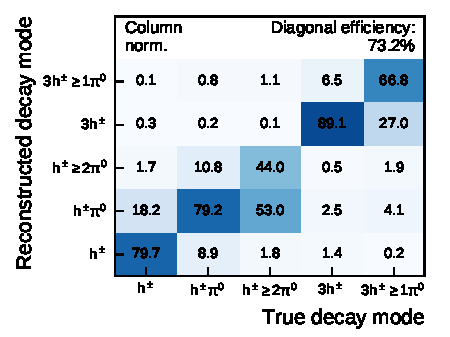
\includegraphics{./figures/decay_mode_classification/mig_mat_pantau.pdf}
    \subcaption{ATLAS default algorithm: \emph{PanTau}}
  \end{subfigure}\hfill
  \begin{subfigure}[t]{0.48\textwidth}
    \centering
    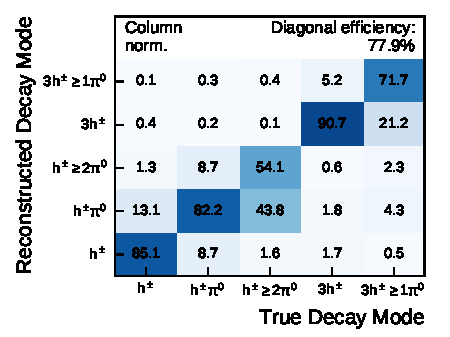
\includegraphics{./figures/decay_mode_classification/mig_mat_baseline_ptcut_1_5.pdf}
    \subcaption{PFO-RNN with neutral $p_{\text{T}}$-cut of
      \SI{1.5}{\giga\electronvolt}}
  \end{subfigure}
  \caption{Migration matrices with normalised columns showing the migration of
    the true decay modes to the reconstructed modes.}
  \label{fig:migmat}
\end{figure}


\begin{figure}[ht]
  \begin{subfigure}[t]{0.48\textwidth}
    \centering
    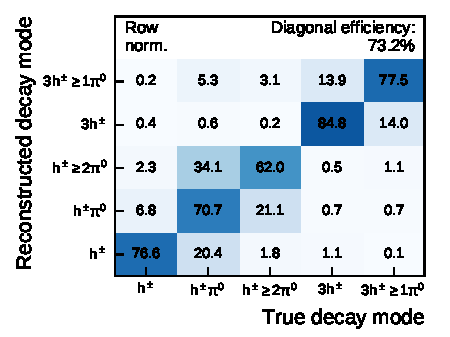
\includegraphics{./figures/decay_mode_classification/comp_mat_pantau.pdf}
    \subcaption{ATLAS default algorithm: \emph{PanTau}}
  \end{subfigure}\hfill
  \begin{subfigure}[t]{0.48\textwidth}
    \centering
    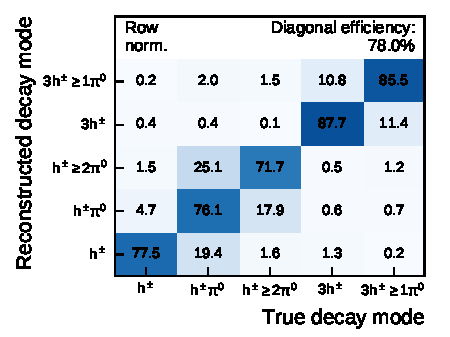
\includegraphics{./figures/decay_mode_classification/comp_mat_baseline_ptcut_1_5.pdf}
    \subcaption{PFO-RNN with neutral $p_{\text{T}}$-cut of
      \SI{1.5}{\giga\electronvolt}}
  \end{subfigure}
  \caption{Composition matrices with normalised rows showing the migration of
    the true decay modes to the reconstructed modes.}
  \label{fig:migmat}
\end{figure}


\begin{figure}[ht]
  \begin{subfigure}[t]{0.48\textwidth}
    \centering
    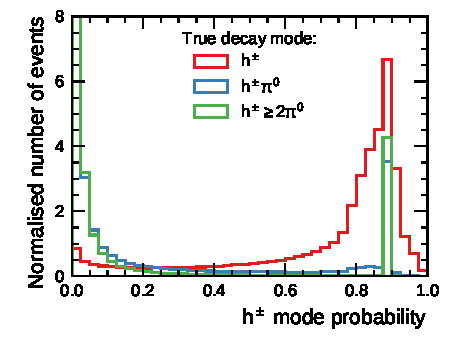
\includegraphics{./figures/decay_mode_classification/mode_proba_baseline_ptcut_1_5_only_1p/proba_1p0n.pdf}
    \subcaption{In most cases the probabilities for modes containing neutral
      pions to be classified as the $h^\pm$ mode are small. However in cases
      where no neutral PFO is reconstructed the probabilities can be large
      \SI{90}{\percent}.}
  \end{subfigure}\hfill
  \begin{subfigure}[t]{0.48\textwidth}
    \centering
    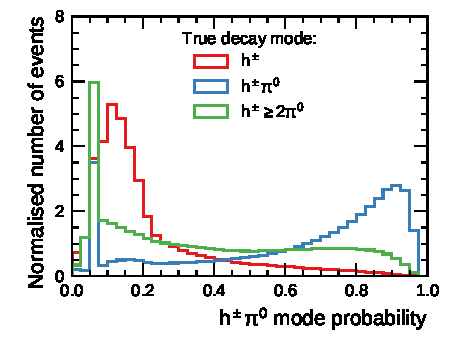
\includegraphics{./figures/decay_mode_classification/mode_proba_baseline_ptcut_1_5_only_1p/proba_1p1n.pdf}
    \subcaption{The discrimination of modes with one neutral and more than one
      neutral pion is difficult. In cases of no reconstructed neutral pions the
      probabilities can be small ($\approx \SI{5}{\percent}$)}
  \end{subfigure}
  \caption{Mode probabilities for the $h^\pm$ and $h^\pm \pi^0$ modes. While
    each tau candidate is assigned a probability for all five decay modes the
    probabilities for the 3-prong modes have been omitted.}
  \label{fig:mode_proba_ptcut}
\end{figure}

'Global' Information attached to every PFO:
\begin{itemize}
\item $p_\text{T}^\text{jet}$
\item $\phi_\text{jet}$
\item $\eta_\text{jet}$
\end{itemize}

Charged PFOs (up to three -- 1 to 1 correspondence with charged tracks):
\begin{itemize}
\item $p_\text{T}^\text{PFO}$
\item $\Delta \phi$: The angle between PFO and jet in the transverse plane.
\item $\Delta \eta = \eta_\text{PFO} - \eta_\text{jet}$: Angle between PFO and
  jet in the pseudorapidity plane
\end{itemize}

Neutral PFOs (Charged PFOs + whats listed here):
\begin{itemize}
\item $S_\text{BDT}^{\pi^0}$ / $p_{\pi^0}$: Probability that the particle flow
  object originates from a neutral pion (ALSO IN BASELINE)
\item $N_\text{shot}$: \texttt{cellBased\_NHitsInEM1} (Number of shots) Sum of
  $N_\text{photon}$ over all shots matched to the cluster (ALSO IN BASELINE)
\item $\langle R^2 \rangle$: Transverse cluster moment
\item $\langle (\eta - \eta_\text{Cluster})^2 \rangle$: Second moment of $\eta$
  with respect to the cluster position.
\item $N_\text{EM1}^\text{pos}$: Number of positive cells in EM1
\item $f_\text{core}$: \texttt{ENG\_FRAC\_CORE} Fraction of energy in the three
  hottest cells in each sampling \todo{Check}
\item $f_\text{EM1} = E_\text{EM1} / E$: Energy fraction in EM2
\end{itemize}

Preprocessing:
\begin{itemize}
\item $p_\text{T}$: log-transform and standard scaling
\item $\eta$, $\phi$: Divided by maximum value ($2.5$ or $\pi$)
\item $\Delta \eta$, $\Delta \phi$: standard scaling
\item Cluster moments: Second\_R, secondEtaWRTClusterPosition, NPosECells\_EM1
  ... standard scaling
\item PI0BDT, NHitsinEM1, ENG\_FRAC\_CORE, energyfrac em2 - no scaling
\end{itemize}

Conversion tracks: same as charged PFOs (but with tracks) \\
Shots: same as charged PFOs (but with shots) \\



% ----------------------------- FIRST DRAFT -------------------------- %
\begin{itemize}
\item Signature of the decay modes (Could be moved to \textit{Theoretical
    Background})
\item Tau Particle Flow \& Currently used decay mode reconstruction (PanTau)
\item RNN
  \begin{itemize}
  \item Only PFOs
  \item PFOs + Cluster-Moments + Conversion Tracks + Shots
  \item Class probabilities, Migration matrices (row + col. norm),
    Efficiency/Purity profiles
  \item Improvements for Higgs CP measurement in
    $H \rightarrow \tau\tau \rightarrow \rho \rho 2\nu$
  \end{itemize}
\end{itemize}

% ------------------------------- ??? ------------------------------ %
\begin{itemize}
\item PFO-RNN

\item Performance when adding conversion tracks

\item Performance when adding shot information

\item Performance when adding hadronic PFOs

\item Performance when adding more cluster information

\end{itemize}

%%% Local Variables:
%%% mode: latex
%%% TeX-master: "mythesis"
%%% End:
